\documentclass{standalone}
\usepackage{tikz}
\begin{document}
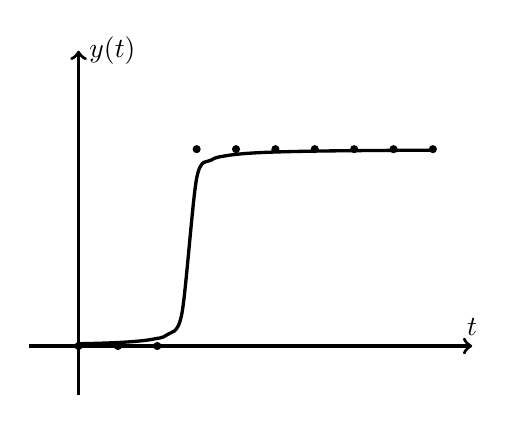
\begin{tikzpicture}[scale=2.5]
    \draw[->,very thick](-0.25,0)--(2,0)node[above]{$t$};
    \draw[->,very thick](0,-0.25)--(0,1.5)node[right]{$y(t)$};

    %\begin{axis}[hide axis,scale=0.1]
    %    \addplot[thick, smooth,domain=0:1]{0.5+rad(atan(50*(x-0.6)))/pi};
    %\end{axis}
    \draw[-,very thick]plot[smooth, domain=0:1.8](\x,{0.5+rad(atan(50*(\x-0.56)))/pi});
    %0.5+rad(atan(50(x-0.6)))/pi
    \filldraw[black](0,0)circle(0.5pt);
    \filldraw[black](0.2,0)circle(0.5pt);
    \filldraw[black](0.4,0)circle(0.5pt);
    \filldraw[black](0.6,1)circle(0.5pt);
    \filldraw[black](0.8,1)circle(0.5pt);
    \filldraw[black](1,1)circle(0.5pt);
    \filldraw[black](1.2,1)circle(0.5pt);
    \filldraw[black](1.4,1)circle(0.5pt);
    \filldraw[black](1.6,1)circle(0.5pt);
    \filldraw[black](1.8,1)circle(0.5pt);
\end{tikzpicture}
\end{document}